\subsubsection{} \textit{AES} шифровка и расшифровка.
\label{sec:eng:performance:aesenc}

Завершающей парой тестовых методов являются методы для шифровки и расшифровки при помощи алгоритма \textit{AES}: \texttt{aesEncrypt} и \texttt{aesDecrypt}. На рисункe \ref{sec:eng:performance:aesenc:ui} представлены результаты измерений шифрования и дешифрования данных при помощи \textit{AES}.

\begin{figure}[h]
  \centering
    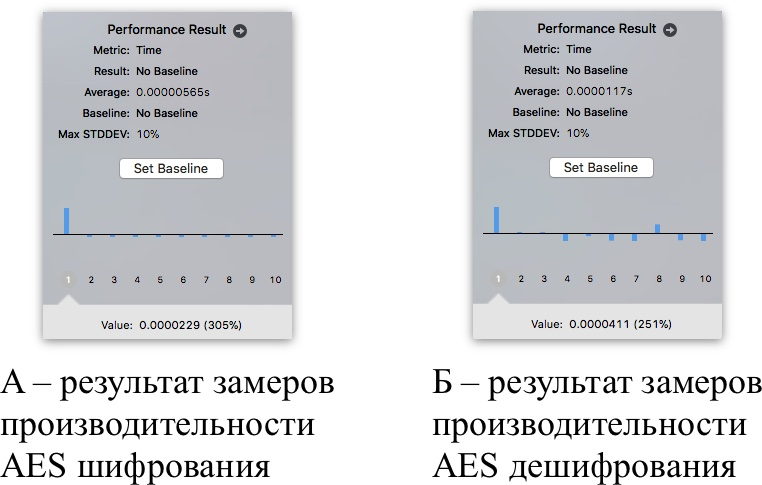
\includegraphics[width=0.75\textwidth]{inc/img/aes_performance_test.jpg}
  \caption{Результаты тестов производительноси модуля AES}
  \label{sec:eng:performance:aesenc:ui}
\end{figure}

\FPeval{\aesEncMesaureMax}{0.000229}
\FPeval{\aesEncMesaureMin}{0.0000448}
\FPeval{\aesEncMesaureAverage}{0.0000565}
\FPeval{\perfAESEnc}{clip(round(((\aesEncryptMaxValue - (\aesEncMesaureMax + \aesEncMesaureMin + \aesEncMesaureAverage) / 3) / \aesEncryptMaxValue) * 100, 2))}

Рассчитаем отклонение от предельно допустимого значения времени, затраченного на шифрование при помощи \textit{AES}, подставив значения в формулу (\ref{perfDifEquation}):
\begin{center}
\(\perfDev = (\num{\aesEncryptMaxValue} - \frac{\num{\aesEncMesaureMax} + \num{\aesEncMesaureMin} + \num{\aesEncMesaureAverage}}{\num{3}}) \cdot \frac{\num{1}}{\num{\aesEncryptMaxValue}} \cdot 100 = \num{\perfAESEnc} \, \text{\%}\)
\end{center}

\FPeval{\aesDecMesaureMax}{0.000411}
\FPeval{\aesDecMesaureMin}{0.000034}
\FPeval{\aesDecMesaureAverage}{0.000117}
\FPeval{\perfAESDec}{clip(round(((\aesDecryptMaxValue - (\aesDecMesaureMax + \aesDecMesaureMin + \aesDecMesaureAverage) / 3) / \aesDecryptMaxValue) * 100, 2))}

Для дешифровки, при помощи алгоритма \textit{AES}, рассчитаем аналогичное значение:
\begin{center}
\(\perfDev = (\num{\aesDecryptMaxValue} - \frac{\num{\aesDecMesaureMax} + \num{\aesDecMesaureMin} + \num{\aesDecMesaureAverage}}{\num{3}}) \cdot \frac{\num{1}}{\num{\aesDecryptMaxValue}} \cdot 100 = \num{\perfAESDec} \, \text{\%}\)
\end{center}
